
\section{Transformer}
\label{sec:transformer}

The \emph{Transformer} architecture is an alternative to RNNs published in 2017,
questioning the need for RNNs following the discovery of the Attention
mechanism~\citep{vaswani:attention}. The original paper presents this
architecture for Machine Translation and introduces two new Attention
mechanisms: \emph{Scaled Dot-Product Attention} and \emph{Multi-Head Attention}.

\subsection{Scaled Dot-Product Attention}
\label{subsec:transformer:scaled:dot-prodct:attention}

\emph{Scaled Dot-Product Attention} provides an Attention score based on a Dot
Product Attention scaled by the square root inverse of the dimension of the
query and key matrices. This scaled version prevents the Dot-Product Attention
mechanism from growing large in magnitude when the dimensionality of the queries
has a high value. Specifically, this high value is due to the multiplication and
the addition of inputs, which push the softmax function into regions where its
gradients are minimal.
\begin{definition}[Scaled Dot-Product Attention]
  Let $Q \in \mathbb{R}^{m\times d_k}$ be the matrix of queries and $K \in
  \mathbb{R}^{n\times d_k}, V \in \mathbb{R}^{m\times d_v}$ be matrices of a set
  of key-value pairs. Mathematically, the the Scaled Dot-Product Attention
  mechanism is defined as follows:
  \begin{equation}
    \mathrm{A}(Q, K, V) = \mathrm{softmax}\left(\frac{QK^T}{\sqrt{d_k}}\right)V
    \label{eq:def:scaled:dot-product:attention}
  \end{equation}

  where $d_k$ is the dimensionality of queries as well as keys and $d_v$ the
  dimensionality of values.
\end{definition}

\subsection{Multi-Head Attention}
\label{subsec:transformer:multi-head:attention}

\emph{Multi-Head Attention} (MHA) is an improved version of the Self-Attention
mechanism where each word not only brings excessive importance to itself, but
pays attention to the interactions with other words. As a result, MHA achieves
better results than Self-Attention, where the latter leads to a loss of
efficiency in the Attention embeddings. Finally, MHA still performs a weighted
average to generate the Attention vector for each token. However, the heads are
this time computed in parallel.

\begin{definition}[Multi-Head Attention]
  Let $f_o: \mathbb{R}^{kd} \to \mathbb{R}^D$ be a linear map, $f_{i,q}, f_{i,
    k}, f_{i, v}: \mathbb{R}^D \to \mathbb{R}^d$ be a three sets of linear maps,
  $\hat{Q} \in \mathbb{R}^{M\times D}$ be a queries vector, and $\hat{K}, \hat{V}
  \in \mathbb{R}^{N\times D}$ be vectors of keys and values. Mathematically, the
  MHA is defined as follows:
  \[
    \textrm{MHA}(\hat{Q}, \hat{K}, \hat{V}) = f_o \left (
      \text{concat} \left (
        \left [
          A \left (
            f_{i,q}(\hat{Q}),
            f_{i,k}(\hat{K}),
            f_{i,v}(\hat{V})
          \right )
          \
          \forall \ i \in 1,\dots, k
        \right ]
      \right )
    \right )
  \]
  where $\text{MHA}(\hat{Q}, \hat{K}, \hat{V}) \in \mathbb{R}^{M \times D}$ is
  the output of the MHA, also known as a \emph{neural function} with $k$-headed
  attention block.
\end{definition}

\subsection{Architecture}
\label{subsec:transformer:architecture}

The Transformer architecture mainly consists of an encoder and a decoder block,
including the Scaled Dot-Product and MHA mechanisms. Specifically, the encoder
and decoder are neural components composed of a stack of $N=6$ identical layers.

Visually, one layer of the Transformer works as follows:
\begin{figure}[!ht]
  \centering
  \subfloat[Encoder\label{fig:transformer:encoder}]{%
    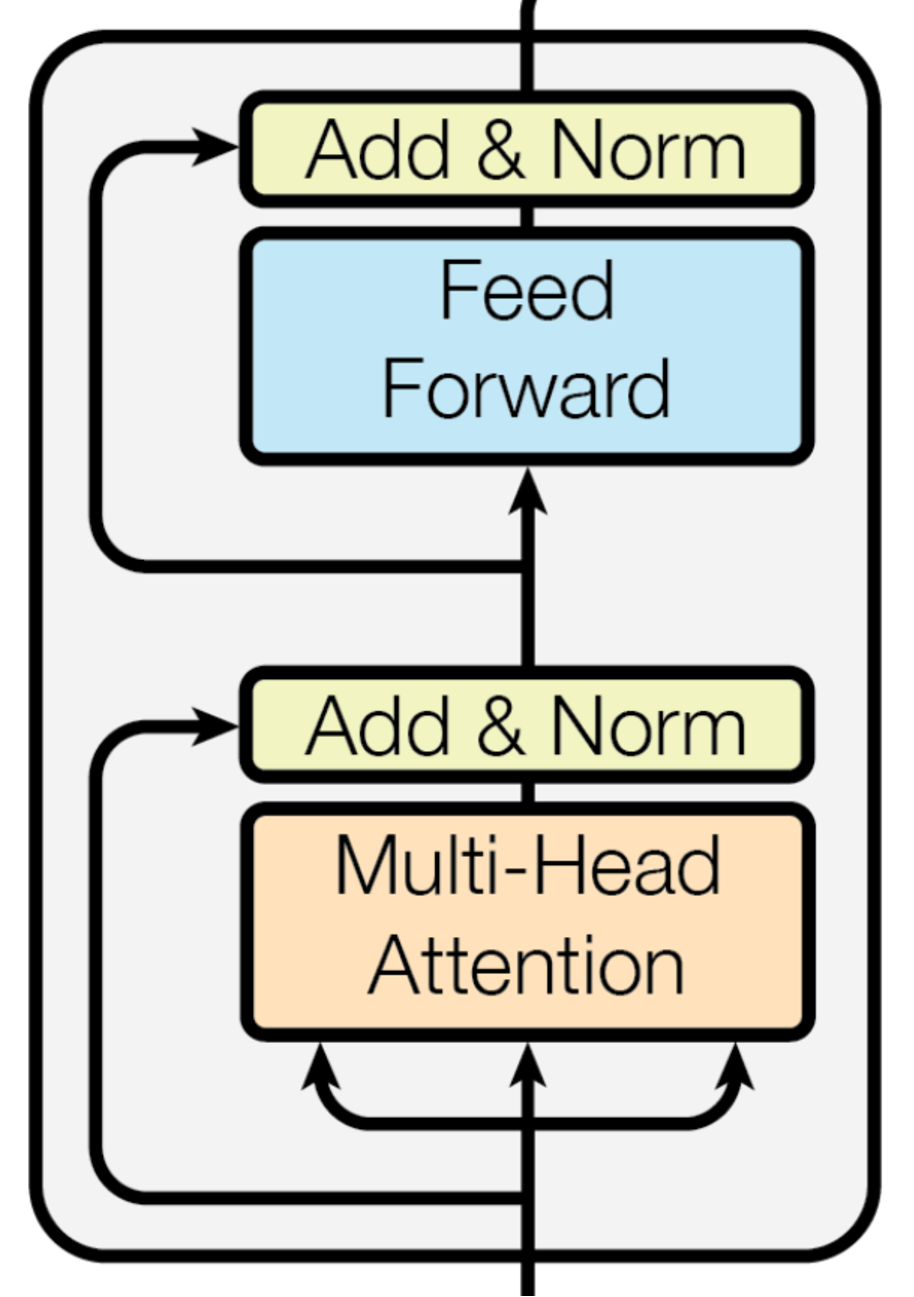
\includegraphics[width=0.23\textwidth]{img/transformer/encoder}
  }
  \quad
  \subfloat[Decoder\label{fig:transformer:decoder}]{%
    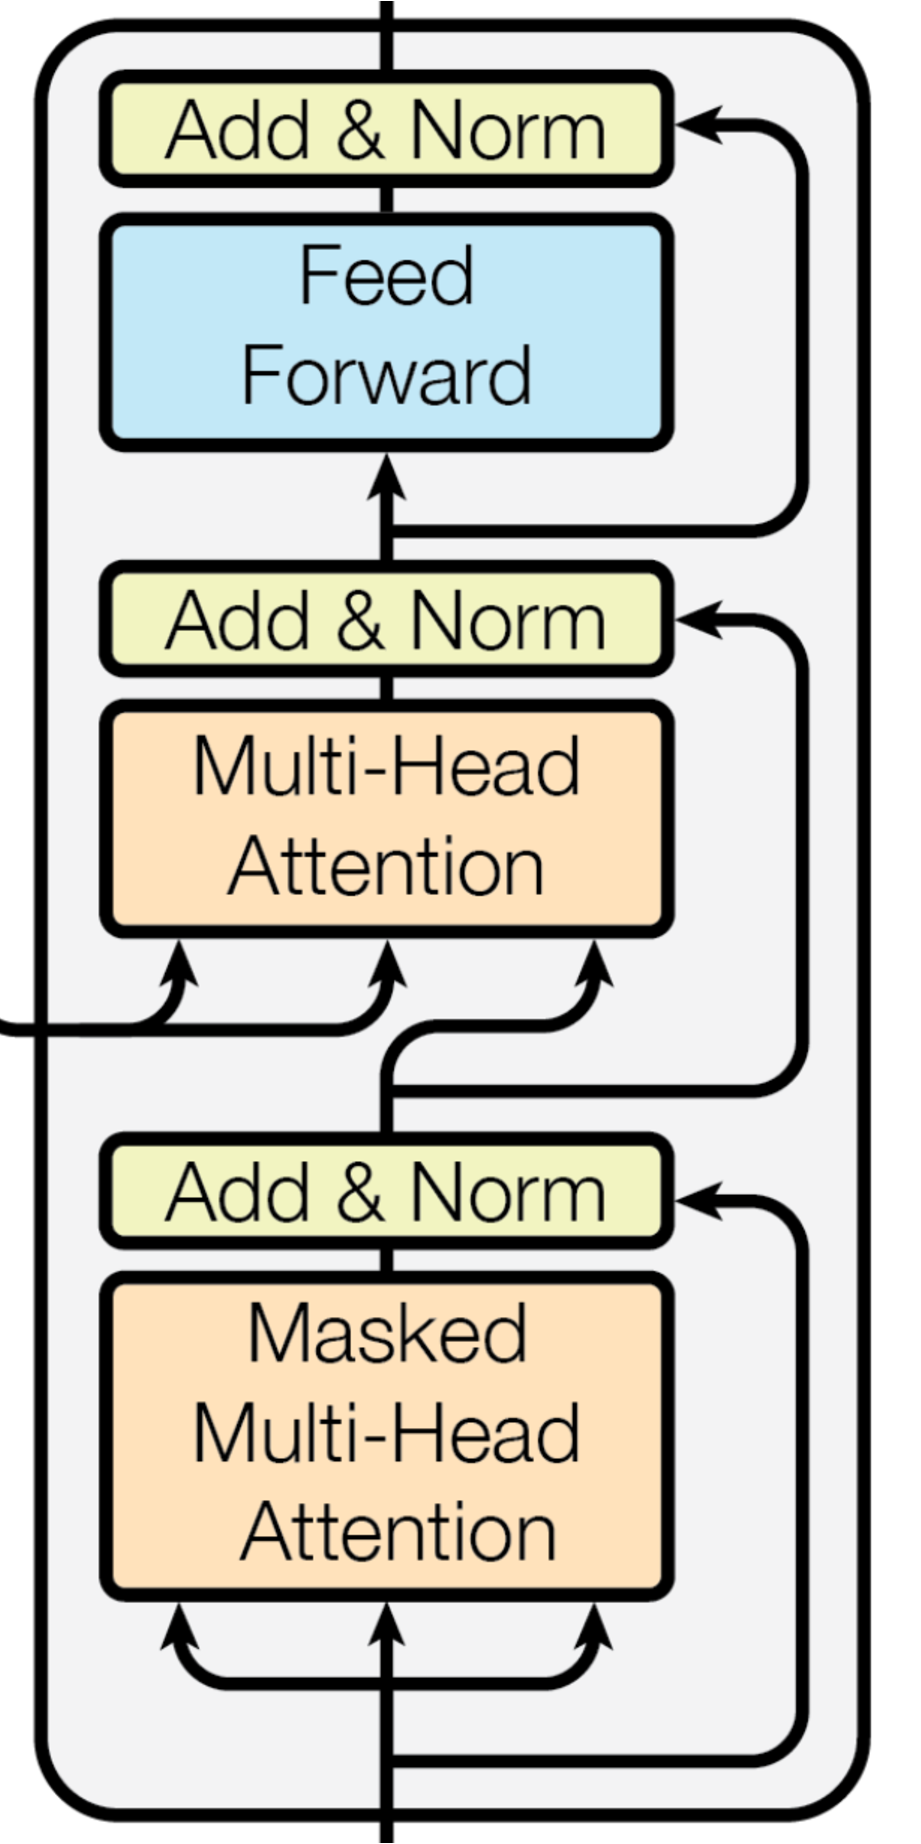
\includegraphics[width=0.23\textwidth]{img/transformer/decoder}
  }
  \caption{One Layer of the Architecture of the Transformer.}
  \label{fig:transformer:architecture:encoder}
  \source{\textsc{Vaswani} et al. -- Attention Is All You Need.}
\end{figure}

In Figure \ref{fig:transformer:encoder}, one layer of the encoder contains two
sub-layers: a MHA mechanism and a position-wise fully connected Feed-Forward
Neural Network (FFN).
\begin{definition}[Feed-Forward Neural Network]
  Let $W_1 + b_1$ and $W_2 + b_2$ be two linear transformations. Mathematically,
  the FFN is defined as follows:
  \begin{equation}
    \mathrm{FFN}(x) = \max\left(0, xW_1 + b_1\right)W_2 + b_2
    \label{eq:def:ffn}
  \end{equation}
  where a ReLU activation function is used.
  \label{def:ffn}
\end{definition}

Moreover, a residual connection followed by a normalization of the layers wraps
each of the two sublayers. Mathematically, the output of every sub-layer is
defined as follows:
\begin{equation}
  \mathrm{LayerNorm}(x + \mathrm{Sublayer}(x))
  \label{eq:output:sub-layer}
\end{equation}
where $\mathrm{Sublayer}(x)$ refers to the implemented function by the sub-layer
itself. \\


\noindent In Figure \ref{fig:transformer:decoder}, the decoder has layers that
differ from the encoder with two sub-layer changes. The first sublayer change is
defined using \emph{Masked MHA} as the first sub-layer to prevent positions from
attending subsequent positions. The last change is adding a new sub-layer,
called \emph{Encoder-Decoder Attention} which performs MHA over the Attention
vectors of the decoder and those of the encoder. The use of this sub-layer makes
it possible to determine the different relationships between these
vectors. Finally, the generated embeddings are sent to a position-wise fully
connected FFN. Like the encoder, each sub-layer is wrapped by a residual
connection followed by a layer normalization.

From then one, the complete architecture of the Transformer is illustrated as follows:
\begin{figure}[!ht]
  \centering
  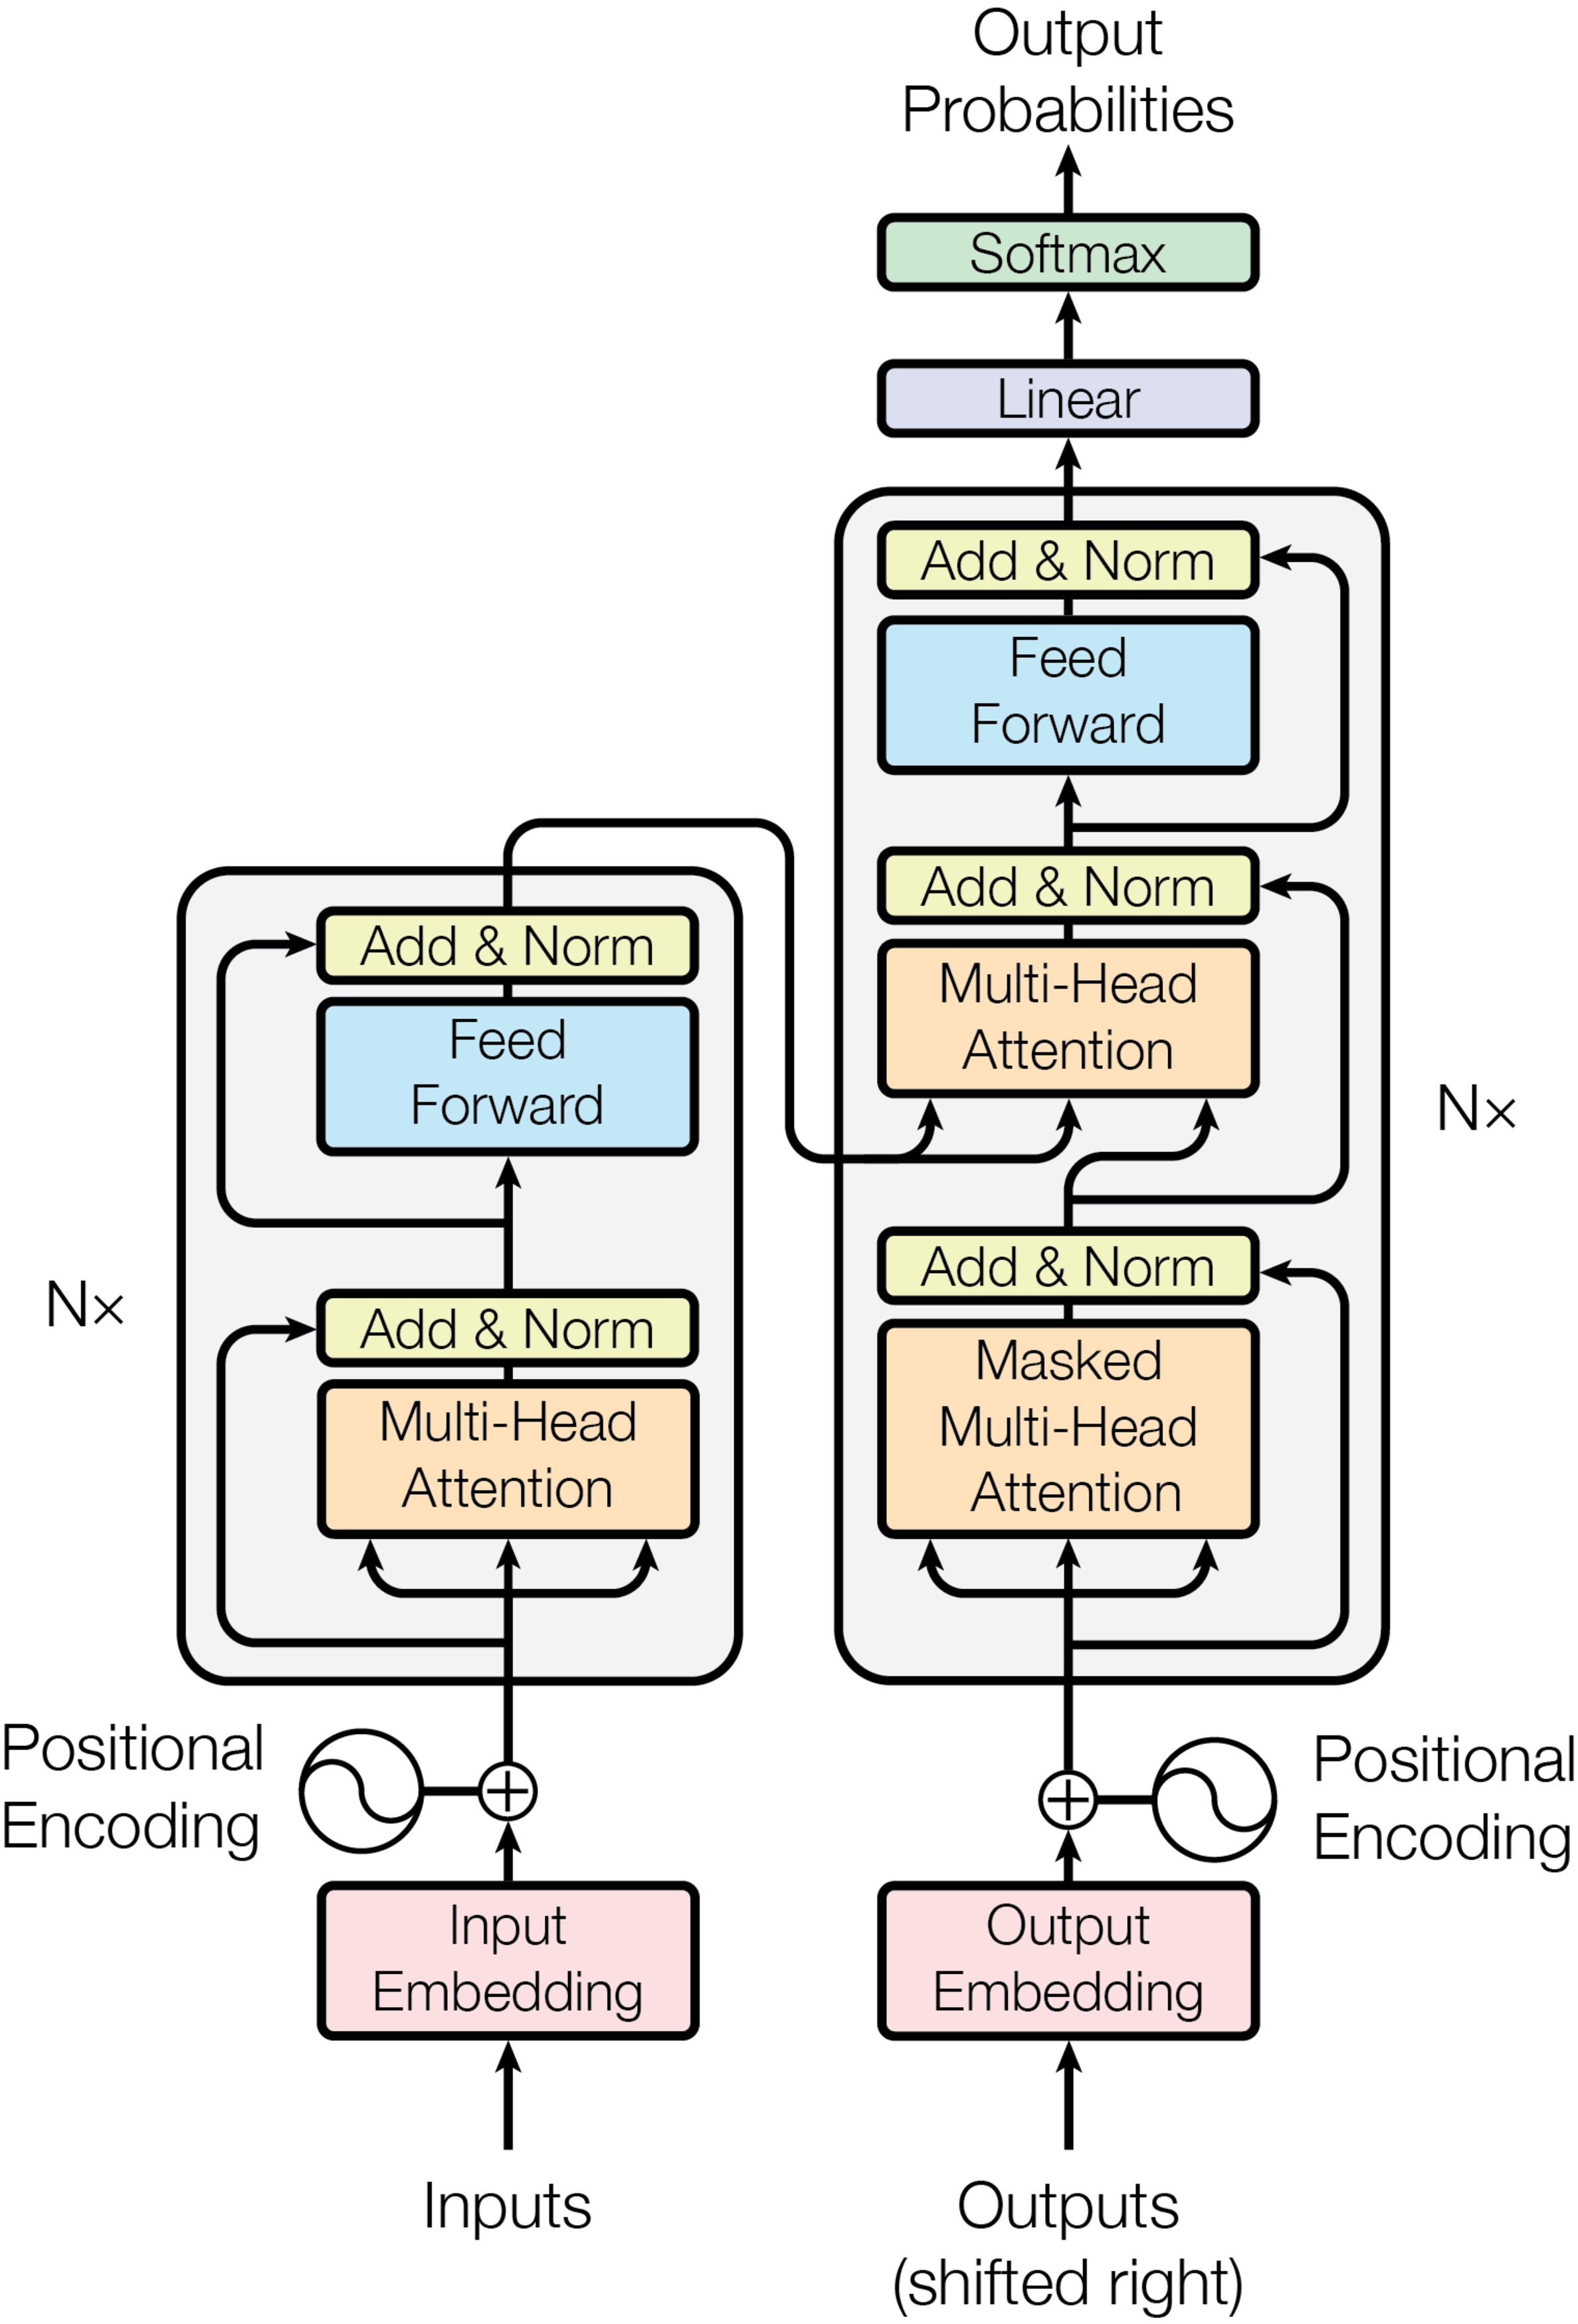
\includegraphics[width=0.6\textwidth]{img/transformer/architecture}
  \caption{Model Architecture of the Transformer.}
  \source{\textsc{Vaswani} et al. -- Attention Is All You Need}
  \label{fig:transformer:architecture}
\end{figure}

\newpage

In Figure \ref{fig:transformer:architecture}, both encoding and decoding take
the sum of the input/output embeddings with positional embedding as
input. Unlike RNNs, Transformer do not have a time step so that input sequences
can be injected simultaneously and converted into input embeddings. Each token
is represented in the embedding space through these input embeddings where
semantically similar tokens are closer than others. However, the decoder has the
particularity of having its input shifted. This shift avoids that a model only
learns to copy the decoder input by allowing a model to predict the target
word/character for position $i$ according to the previous one from 1 to $i-1$.

At last, the output of the decoding layer is sent to a linear layer. This layer
is nothing more than an FFN layer whose objective is to extend the dimension of
this vector to the number of words of the language concerned. Once expanded,
this vector is submitted to a softmax activation function to transform it into a
probability distribution and predict the next word according to the word with
the highest probability. Afterward, this decoding process is iterated several
times until the end-of-sentence token is generated.

\subsection{Positional Encoding}
\label{subsec:transformer:positional:encoding}

Considering that the transformer has no recurrence or convolution mechanism, the
architecture cannot know the order in an input sequence. From then on, the
transformer encodes the same meaning for different sentences. The easiest way to
take this context into account is to encode these positions as one-hot features.
\begin{definition}[Positional Encoding as One-Hot Features]
  Let $x \in \mathbb{R}^{n \times d}$ be a matrice of sequentially ordered data
  along the $n$-dimensional axis, and $e_k$ be a $k$'th standard basis vector in
  $\mathbb{R}^n$. Mathematically, the $z \in \mathbb{R}^{n \times d}$ learned
  combined representation is defined as follows:
  \begin{equation}
    \mathrm{z}_k = W^T_zReLU\left(W_x^Tx_k + W_e^Te_k\right), W_x \in
    \mathbb{R}^{dim(x)\times m}, W_e \in \mathbb{R}^{n\times m}, W_z \in \mathbb{R}^{m\times d}
    \label{eq:def:positional:encoding:one:hot}
  \end{equation}
  \label{def:positional:encoding:one:hot}
\end{definition}

\noindent Another approach for positional encoding is to build distinct
representations of inputs and positions~\citep{gehring}. Despite these existing
approaches to differentiate meanings, the original Transformer paper uses a
sinusoid-wave-based positional encoding to inject absolute positional
information of tokens into the sequence.

\begin{definition}[Positional Encoding by \textsc{Vaswani} et al.]
  Let $d_{model}$ be the embedding dimension of words, and $pos \in \left[0, L -
    1\right]$ be the position of a $w$ word in the $w = (w_0,\dotsc,w_{L-1})$ input
  sequence. Mathematically, the positional encoding of $w$ is defined as follows:
  \begin{align}
    \mathrm{PE}(pos,i) = \begin{cases}
      \sin\displaystyle\left(\frac{pos}{10000^{2i/d_{model}}}\right)\,, & i = 2k \\\\
      \cos\displaystyle{\left(\frac{pos}{10000^{2i/d_{model}}}\right)}\,, & i = 2k + 1
    \end{cases} \   k \in \mathbb{N}
    \label{eq:positional:encoding}
  \end{align}

  where the positional encoding follows a specific, learned pattern to identify
  word position or the distance between words in the sequence~\citep{alammar}.  In
  Equation \ref{eq:positional:encoding}, the sinusoidal representation works as
  well as a learned representation and better generalizes sequences that are
  longer than the training sequences~\citep{vaswani:attention}.
\end{definition}

%%% Local Variables:
%%% mode: latex
%%% TeX-master: "../../report"
%%% End:
